% ----------- Cover Master Thesis Faculty of Sciences ---------------
% This document should be compiled with pdflatex.  If you want to use
% latex to compile to dvi/ps, you have to convert the images to (e)ps
%                           -- December 2012
% -------------------------------------------------------------------


% ----------------------- Cover --------------------------------------
% Please fill in:
% - The title and subtitle (if applicable)
%         to include a formula in the title or subtitle
%         use  \form{$...$}
% - Your name
% - Your (co)supervisor, mentor (if applicable)
% - Your master
% - The academic year
% --------------------------------------------------------------------
\thispagestyle{empty}
\newcommand{\form}[1]{\scalebox{1.087}{\boldmath{#1}}}
\sffamily
%
\begin{textblock}{191}(-24,-11)
\colorbox{green}{\hspace{139mm}\ \parbox[c][18truemm]{60mm}{\textcolor{white}{FACULTY OF ENGINEERING}}}
\end{textblock}
%
\begin{textblock}{70}(-18,-19)
\textblockcolour{}
\includegraphics*[height=19.8truemm]{./src/LogoKULeuven}
\end{textblock}
%
\begin{textblock}{160}(-6,63)
\textblockcolour{}
\vspace{-\parskip}
\flushleft
\fontsize{40}{42}\selectfont \textcolor{bluetitle}{Support Vector Machines Report }\\[1.5mm]
%\fontsize{20}{22}\selectfont Subtitle \form{$S=\pi r^2$\textsl{(optional)}}
\end{textblock}
%
\vspace{-\parskip}
\begin{textblock}{160}(7,100)
%\includegraphics[scale = 0.8]{/home/moritz/uni/dataMining/exercise2/report2/src/tikz/networkavg1.tex}
%\includegraphics[scale = 0.8]{/home/moritz/uni/dataMining/exercise5/report/tikz/vapHardPloySep2.tex}
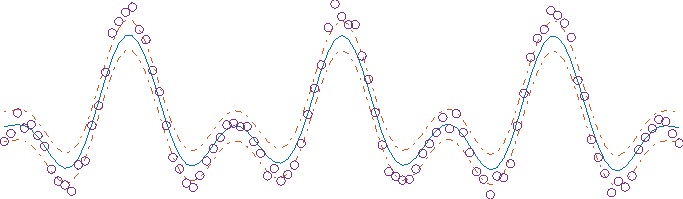
\includegraphics[scale=1.2]{/home/moritz/uni/svm/linkReport/src/titleFun.pdf}
\end{textblock}
%
\begin{textblock}{160}(8,153)
\textblockcolour{}
\vspace{-\parskip}
\flushright
\fontsize{14}{16}\selectfont \textbf{Moritz Wolter}
\end{textblock}
%
%\begin{textblock}{70}(-6,191)
%\textblockcolour{}
%\vspace{-\parskip}
%flushleft
%Supervisor: Prof. A. Xyz\\[-2pt]
%\textcolor{blueaff}{Affiliation \textsl{(optional)}}\\[5pt]
%Co-supervisor: \textsl{(optional)}\\[-2pt]
%\textcolor{blueaff}{Affiliation \textsl{(optional)}}\\[5pt]
%Mentor: \textsl{(optional)}\\[-2pt]
%\textcolor{blueaff}{Affiliation \textsl{(optional)}}\\
%\end{textblock}
%
%\begin{textblock}{160}(8,191)
%\textblockcolour{}
%\vspace{-\parskip}
%\flushright
%Thesis presented in\\[4.5pt]
%fulfillment of the requirements\\[4.5pt]
%for the degree of Master of Science\\[4.5pt]
%in Xxx\\
%\end{textblock}
%%
%\begin{textblock}{160}(8,232)
%\textblockcolour{}
%\vspace{-\parskip}
%flushright
%Academic year 20XX-20XX
%\end{textblock}
%
%\begin{textblock}{191}(-24,248)
%{\color{blueline}\rule{550pt}{5.5pt}}
%\end{textblock}
%
\rmfamily
